% Section 10: Hermitian and Positive Definite Matrices  (original handwritten pages 77--84)
% ===== Page 77 =====
\section{Hermitian and Positive Definite Matrices}\label{sec:hermitian}
\syllabusweek{Week 13 --- Hermitian, positive definite and positive semi-definite matrices}

\subsection{Hermitian Matrices and Their Eigenstructure}\label{ss:hermitian-props}

\begin{itemize}[label=$\ast$]
\item\leavevmode\origpage{77}An $n\times n$, in general, complex matrix $A\in\C^{n\times n}$ is called \term{Hermitian} iff
\[
\bar A^{T}=A, \qquad\text{i.e.}\qquad A\Hm=A,
\]
where $\bar{\ }^{T}\triangleq{}^{H}$: the complex conjugate transpose is denoted as Hermitian.
\item If $A\in\R^{n\times n}$:
\[
A\T=A:\ \text{Symmetric matrices are Hermitian.}
\]
\item Example:
\[
\bmat{2&1\\1&2},\qquad \lambda_1=3,\ \lambda_2=1,\qquad e_1=\bmat{1\\1},\quad e_2=\bmat{1\\-1}
\]
\item In addition to being linearly independent, eigenvectors of Hermitian matrices (for distinct eigenvalues) are \key{\underline{orthogonal}}.
\item \key{Eigenvalues are always real} in Hermitian matrices.
\end{itemize}

\begin{theorem}
Let $A\in\C^{n\times n}$ be Hermitian. Then \key{$\inner{x}{Ax}$ is real $\forall x\in\C^n$}.
\end{theorem}

$\ast$ $\inner{x}{y}=y\Hm x$: $\ell_2$-inner product. Properties:
\begin{align*}
&\inner{\alpha x}{y}=\alpha\inner{x}{y}, & &\inner{x}{x}\text{ is real},\\
&\inner{x}{\alpha y}=\bar\alpha\inner{x}{y}, & &\inner{x}{x}\geq0\ \ \forall x\in\C^n,\\
&\inner{x}{y}=\overline{\inner{y}{x}}, & &\inner{x}{x}=0\iff x=0,
\end{align*}
\[
\inner{x}{Ay}=(Ay)\Hm x=y\Hm(A\Hm x)=\inner{A\Hm x}{y}.
\]

\begin{proof}[Proof]
\[
\inner{x}{Ax}=(Ax)\Hm x=x\Hm A\Hm x\overset{A\Hm=A}{=}x\Hm Ax:\ \text{\term{Quadratic Form}}
\]
\begin{align*}
\overline{\inner{x}{Ax}}&=\inner{Ax}{x}\\
&=\inner{x}{A\Hm x}\qquad\text{(identity above for $A\Hm$, with $y=x$)}\\
&=\inner{x}{Ax}\qquad\text{if $A$ is Hermitian}
\end{align*}
The complex conjugate is equal to itself $\Rightarrow$ $\inner{x}{Ax}$ is real.
\end{proof}

% ===== Page 78 =====
\begin{theorem}
\leavevmode\origpage{78}If $A$ is Hermitian, then \key{its eigenvalues are all real}.
\end{theorem}
\begin{proof}[Proof]
$\lambda_i, e_i$: one eigenvalue of $A$ and corresponding eigenvector.
\begin{align*}
\inner{x}{Ax}\Big|_{x=e_i}&=\inner{e_i}{Ae_i}\\
&=\inner{A\Hm e_i}{e_i}\\
&=\inner{Ae_i}{e_i}\\
&=\inner{\lambda_ie_i}{e_i}\\
&=\lambda_i\underbrace{\inner{e_i}{e_i}}_{\text{always real}}\ \Rightarrow\ \text{should be real}
\end{align*}
\[
\Rightarrow\ \underline{\underline{\lambda_i\text{ is real}}}
\]
\explain{By the previous theorem $\inner{e_i}{Ae_i}$ is real. Also, since $e_i\neq0$, we have $\inner{e_i}{e_i}=\norm{e_i}_2^2>0$. Hence $\lambda_i=\inner{e_i}{Ae_i}/\inner{e_i}{e_i}$ is real.}
\end{proof}

\begin{theorem}
Let $A$ be Hermitian, and let $\lambda_i,\lambda_j$ be two distinct eigenvalues of $A$ with eigenvectors $e_i$ and $e_j$. Then \key{$e_i$ and $e_j$ are orthogonal}:
\[
\lambda_i\neq\lambda_j\ \Rightarrow\ \inner{e_i}{e_j}=0
\]
% corrected: notes had "lambda_i = lambda_j"; the hypothesis is lambda_i != lambda_j
\end{theorem}
\begin{proof}[Proof]
\[
\begin{array}{c@{\ }c@{\ }c@{\ }c@{\ }c}
\inner{e_i}{Ae_j} &=& \inner{e_i}{\lambda_je_j} &=& \lambda_j\inner{e_i}{e_j}\\
\shortparallel & & & & \\
\inner{Ae_i}{e_j} &=& \inner{\lambda_ie_i}{e_j} &=& \lambda_i\inner{e_i}{e_j}
\end{array}
\]
\begin{align*}
\lambda_j\inner{e_i}{e_j}&=\lambda_i\inner{e_i}{e_j}\\
\underbrace{(\lambda_i-\lambda_j)}_{\neq0}\underbrace{\inner{e_i}{e_j}}_{=0}&=0
\end{align*}
\explain{Top row: $\inner{e_i}{\lambda_je_j}=\bar\lambda_j\inner{e_i}{e_j}=\lambda_j\inner{e_i}{e_j}$ since $\lambda_j$ is real. Left equality: $\inner{e_i}{Ae_j}=\inner{A\Hm e_i}{e_j}=\inner{Ae_i}{e_j}$.}
Hence
\[
\Null(A-\lambda_iI)\perp\Null(A-\lambda_jI)\ :\ \text{Eigenspaces are also orthogonal.}
\]
\end{proof}

% ===== Page 79 =====
\begin{theorem}
\leavevmode\origpage{79}Let $A$ be Hermitian. Then its minimal polynomial is
\[
m(s)=(s-\lambda_1)(s-\lambda_2)\cdots(s-\lambda_k)
\]
when $A$ has $k$ distinct eigenvalues $\lambda_1,\lambda_2,\dots,\lambda_k$, i.e.\ \key{$m_i=1$ $\forall i$}.
\end{theorem}
In general:
\begin{align*}
d(s)&=(s-\lambda_1)^{r_1}(s-\lambda_2)^{r_2}\cdots(s-\lambda_k)^{r_k}\\
m(s)&=(s-\lambda_1)^{m_1}(s-\lambda_2)^{m_2}\cdots(s-\lambda_k)^{m_k},\qquad 1\leq m_i\leq r_i\ \text{in general case.}
\end{align*}
% corrected: notes had "1 <= m_i <= r_k" (meaning r_i)

\begin{proof}[Proof]
Let $\Sigma_i=A-\lambda_iI$. In general
\[
\Null(\Sigma_i)\subsetneq\Null(\Sigma_i^2)\subsetneq\cdots\subsetneq\Null(\Sigma_i^{m_i})=\Null(\Sigma_i^{m_i+1}).
\]
\[
\Null(\Sigma_i)=\Null(\Sigma_i^2)\ :\ \text{Theorem's Claim.}
\]
We show both inclusions.
\[
\Null(\Sigma_i)\subset\Null(\Sigma_i^2)\colon\quad \Sigma_ix=0\ \text{implies}\ \Sigma_i(\Sigma_ix)=0 \qquad\checkmark
\]
$\Null(\Sigma_i^2)\subset\Null(\Sigma_i)$:
\begin{align*}
x\in\Null(\Sigma_i^2)\ &\Rightarrow\ \Sigma_i^2x=0\\
&\Rightarrow\ \inner{x}{\Sigma_i^2x}=0\\
&\Rightarrow\ \inner{x}{\Sigma_i\Sigma_ix}=0\\
&\Rightarrow\ \inner{\Sigma_i\Hm x}{\Sigma_ix}=0\\
&\Rightarrow\ \inner{\Sigma_ix}{\Sigma_ix}=0\\
&\Rightarrow\ \norm{\Sigma_ix}_2^2=0\ \Rightarrow\ \Sigma_ix=0\ \Rightarrow\ x\in\Null(\Sigma_i)
\end{align*}
\explain{Used: $\Sigma_i\Hm=(A-\lambda_iI)\Hm=A\Hm-\bar\lambda_iI\Hm=A-\lambda_iI=\Sigma_i$ (since $\lambda_i$ is real).}
Hence $\Null(\Sigma_i)=\Null(\Sigma_i^2)$, the chain of null spaces stops at the first step, and $m_i=1$ for every $i$.
\end{proof}

\begin{itemize}[label=$\ast$]
\item Direct sum decompositions:
\begin{align*}
\C^n&=\Null(\Sigma_1^{m_1})\oplus\Null(\Sigma_2^{m_2})\oplus\cdots\oplus\Null(\Sigma_k^{m_k})\\
\C^n&=\Null(\Sigma_1)\overset{\perp}{\oplus}\Null(\Sigma_2)\overset{\perp}{\oplus}\cdots\overset{\perp}{\oplus}\Null(\Sigma_k)
\end{align*}
\explain{Orthogonal as every subspace defines a unique eigenspace: since $m_i=1$, $\Null(\Sigma_i^{m_i})=\Null(\Sigma_i)$ is the eigenspace of $\lambda_i$, and eigenspaces of distinct eigenvalues are orthogonal.}
\item $m_i$ is the size of the largest Jordan block for $\lambda_i$.
% ===== Page 80 =====
\item\leavevmode\origpage{80}For a Hermitian matrix:
\[
\begin{array}{ccc}
\Null(\Sigma_i)&=&\Null(\Sigma_i^2)\\
\scriptstyle\dim r_i&&\scriptstyle\dim r_i
\end{array}
\qquad\Rightarrow\qquad
\begin{aligned}
&(\#\text{ of JB's for }\lambda_i)=r_i\\
&(\#\text{ of JB's with size}\geq2\text{ for }\lambda_i)=0\\
&\Rightarrow\ r_i\text{ JB's of size }1\text{ for }\lambda_i
\end{aligned}
\]
\[
J=\left[\begin{array}{ccc|ccc|c|ccc}
\lambda_1&0&0&&&&&&&\\
0&\lambda_1&0&&&&&&&\\
&&\lambda_1&&&&&&&\\\hline
&&&\lambda_2&0&0&&&&\\
&&&&\lambda_2&0&&&&\\
&&&0&&\lambda_2&&&&\\\hline
&&&&&&\ddots&&&\\\hline
&&&&&&&\lambda_k&0&0\\
&&&&&&&&\lambda_k&0\\
&&&&&&&0&&\lambda_k
\end{array}\right]
\ :\ \text{diagonal matrix.}
\]
\explain{The $\lambda_1$ block is $r_1\times r_1$, the $\lambda_2$ block $r_2\times r_2$, \dots, the $\lambda_k$ block $r_k\times r_k$.}
\item $J$ is diagonal for a Hermitian matrix. \key{Any Hermitian matrix is diagonalizable}:
\[
J=\bmat{\lambda_1I_{r_1\times r_1}&&&\\&\lambda_2I_{r_2\times r_2}&&\\&&\ddots&\\&&&\lambda_kI_{r_k\times r_k}}_{n\times n}
\]
\item Any Hermitian matrix has $n$ linearly independent eigenvectors.
\item For diagonalization with orthonormal eigenvectors (unitary diagonalization), we need to have:
\begin{align*}
&N\Hm N=NN\Hm\ :\ \text{\term{normal matrix} (outside the scope of the course)},\\
&N\Hm N=N^2=NN\Hm\ \text{for Hermitian matrices (inherently normal).}
\end{align*}
% corrected: notes had "For diagonalization, we need" (normality is needed for unitary diagonalization, not for diagonalization in general) and "N^2 = N^2" (meaning N^H N = N^2 = N N^H when N^H = N)
\end{itemize}

\sep
\paragraph{Summary.}
\[
\text{Hermitian}\ \Longrightarrow\
\begin{array}{l}
\lambda_i\text{'s are real}\\
e_i\perp e_j\text{ when }\lambda_i\neq\lambda_j\\
\left.\begin{array}{@{}l}
m_i=1\ \ \forall i\\
J\text{ is diagonal}\\
n\text{ linearly independent eigenvectors}
\end{array}\right\}
\end{array}
\ \Longleftarrow\ \begin{array}{l}A\text{ is normal}\\ \text{(for these 3 statements)}\end{array}
\]
% corrected: notes had "<=> A is normal"; normality implies the three statements, but a diagonalizable matrix need not be normal
\explain{The three bracketed statements are equivalent, and they mean diagonalizability.}
\explain{$\not\Longleftarrow$: the reverse implication (to Hermitian) is not true!}

\begin{insight}[Hermitian, normal, diagonalizable]
\begin{itemize}[nosep]
\item Hermitian $\Rightarrow$ normal $\Rightarrow$ diagonalizable; neither arrow can be reversed.
\item $A$ is normal $\iff$ $A$ has $n$ \emph{orthonormal} eigenvectors $\iff$ $A=U\Lambda U\Hm$ with $U$ unitary. Hermitian matrices are exactly the normal matrices with real eigenvalues.
\item Counterexamples: $\bmat{0&1\\-1&0}$ is normal (and diagonalizable over $\C$, eigenvalues $\pm j$) but not Hermitian; $\bmat{1&1\\0&2}$ is diagonalizable (two distinct eigenvalues, so $m_i=1$) but not normal, its eigenvectors $\bmat{1\\0}$ and $\bmat{1\\1}$ are not orthogonal.
\end{itemize}
\end{insight}

% ===== Page 81 =====
\subsection{Unitary Diagonalization}\label{ss:unitary}
\origpage{81}%
\begin{theorem}[Unitary diagonalization]
Let $A$ be an $n\times n$ Hermitian matrix. Then, \key{there exists a unitary matrix $P$} s.t.
\[
J = P\Hm A P .
\]
\end{theorem}
\begin{insight}[What $J$ looks like here]
For a Hermitian matrix the Jordan form $J$ is \emph{diagonal} with \emph{real} entries: the eigenvalues of $A=A\Hm$ are real, and $A$ is always diagonalizable (every eigenvalue has $m_j=1$ in the minimal polynomial). The theorem adds that the diagonalizing matrix can be chosen \emph{unitary}, i.e.\ $P^{-1}=P\Hm$, so that $A = PJP\Hm$ (unitary diagonalization).
\end{insight}
\begin{itemize}
\item[$\star$] \term{Unitary matrix}: $P^{-1} = P\Hm$.
\item[$\rightarrow$] \term{Orthogonal matrix} (real-valued unitary matrix): $P^{-1} = P\T$.
\item[$\star$] $P^{-1}P = PP^{-1} = I$, \quad i.e.\ \quad $P\Hm P = PP\Hm = I$.
\end{itemize}

\sep
\paragraph{Columns of a unitary matrix.}
\[
P = \bigl[\, p_1 \;\vdots\; p_2 \;\vdots\; \cdots \;\vdots\; p_n \,\bigr],
\qquad
P\Hm = \bmat{p_1\Hm\\ p_2\Hm\\ \vdots\\ p_n\Hm}
\]
\begin{align*}
P\Hm P &= \bmat{p_1\Hm\\ p_2\Hm\\ \vdots\\ p_n\Hm}\bigl[\, p_1 \;\vdots\; p_2 \;\vdots\; \cdots \;\vdots\; p_n \,\bigr]
= \bmat{p_1\Hm p_1 & p_1\Hm p_2 & \cdots & p_1\Hm p_n\\
p_2\Hm p_1 & p_2\Hm p_2 & \cdots & p_2\Hm p_n\\
\vdots & & & \vdots\\
p_n\Hm p_1 & & & p_n\Hm p_n}\\
&= \bmat{\inner{p_1}{p_1} & \inner{p_2}{p_1} & \cdots & \inner{p_n}{p_1}\\
\inner{p_1}{p_2} & & & \vdots\\
\vdots & & & \\
\inner{p_1}{p_n} & & & \inner{p_n}{p_n}}
\end{align*}
\explain{All entries are inner products, similar to a Gram matrix.}
$\Rightarrow$ \key{Columns of $P$ are orthonormal!}
\[
\inner{p_i}{p_j} = \delta_{ij} = \begin{cases} 1, & i=j\\ 0, & i\neq j\end{cases}
\]

% ===== Page 82 =====
\origpage{82}
\paragraph{Rows of a unitary matrix.}
\begingroup\renewcommand{\arraystretch}{1.25}%
\[
P = \bmat{r_1\\ \hline r_2\\ \hline \vdots\\ \hline r_n},
\qquad
\underbrace{\bmat{r_1\\ r_2\\ \vdots\\ r_n}}_{P}
\underbrace{\bigl[\, r_1\Hm \;\vdots\; r_2\Hm \;\vdots\; \cdots \;\vdots\; r_n\Hm \,\bigr]}_{P\Hm} = I
\]\endgroup
$\Rightarrow$ \key{Rows are also orthonormal!}

\begin{proof}[Proof (kind of proof, not an actual one)]
$A$ is Hermitian, $A\in\C^{5\times 5}$; $\lambda_1,\lambda_2$ are eigenvalues of $A$, $\lambda_1\neq\lambda_2$, and $\Sigma_j = A-\lambda_jI$:
\begin{align*}
d(s) &= (s-\lambda_1)^2(s-\lambda_2)^3\\
m(s) &= (s-\lambda_1)(s-\lambda_2)
\end{align*}
\[
\C^5 = \underbrace{\Null(\Sigma_1)}_{\dim 2} \overset{\perp}{\oplus} \underbrace{\Null(\Sigma_2)}_{\dim 3}
\]
\begin{center}
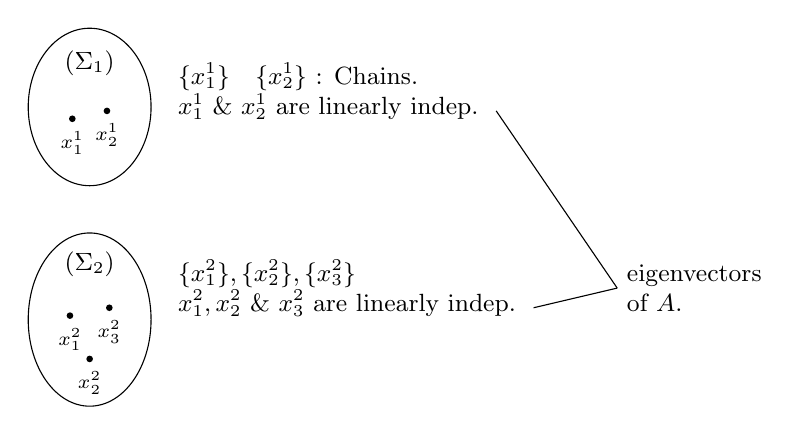
\begin{tikzpicture}[font=\small]
% ellipse N(Sigma_1)
\draw (0,0) ellipse (0.78 and 1.0);
\node at (0,0.55) {$\Null(\Sigma_1)$};
\fill (-0.22,-0.15) circle (1.2pt) node[below=1pt] {\scriptsize $x_1^1$};
\fill (0.22,-0.05) circle (1.2pt) node[below=1pt] {\scriptsize $x_2^1$};
\node[right,align=left] (t1) at (1.0,0.2) {$\{x_1^1\}\quad\{x_2^1\}$ : Chains.\\ $x_1^1$ \& $x_2^1$ are linearly indep.};
% ellipse N(Sigma_2)
\draw (0,-2.7) ellipse (0.78 and 1.1);
\node at (0,-2.0) {$\Null(\Sigma_2)$};
\fill (-0.25,-2.65) circle (1.2pt) node[below=1pt] {\scriptsize $x_1^2$};
\fill (0.25,-2.55) circle (1.2pt) node[below=1pt] {\scriptsize $x_3^2$};
\fill (0,-3.2) circle (1.2pt) node[below=1pt] {\scriptsize $x_2^2$};
\node[right,align=left] (t2) at (1.0,-2.3) {$\{x_1^2\},\{x_2^2\},\{x_3^2\}$\\ $x_1^2, x_2^2$ \& $x_3^2$ are linearly indep.};
% "eigenvectors of A" bracket
\draw (t1.east) ++(0.1,-0.25) -- (6.7,-2.3) coordinate (k);
\draw (t2.east) ++(0.1,-0.25) -- (k);
\node[right,align=left] at (k) {eigenvectors\\ of $A$.};
\end{tikzpicture}
\end{center}
\[
J = \bmat{\lambda_1 & & & & \\ & \lambda_1 & & \text{\Large 0} & \\ & & \lambda_2 & & \\ & \text{\Large 0} & & \lambda_2 & \\ & & & & \lambda_2}
\]
\[
P = \bigl[\, x_1^1 \;\vdots\; x_2^1 \;\vdots\; x_1^2 \;\vdots\; x_2^2 \;\vdots\; x_3^2 \,\bigr]_{5\times 5}
\]
$P$ is not directly unitary. The theorem states that there exists a unitary matrix $P$, which can be found. How can we convert $P$ to a unitary one?
\[
\underbrace{x_1^1\quad x_2^1}\qquad \underbrace{x_1^2\quad x_2^2\quad x_3^2}
\]
\explain{Vectors are orthogonal between the two sets. Vectors inside the sets are not necessarily orthogonal.}
\begin{insight}[Why eigenvectors of different eigenvalues are orthogonal]
If $Ax=\lambda_1x$, $Ay=\lambda_2y$ with $A=A\Hm$ (so $\lambda_1,\lambda_2\in\R$), then
\[
\lambda_1\, y\Hm x = y\Hm A x = (A y)\Hm x = \lambda_2\, y\Hm x
\ \Rightarrow\ (\lambda_1-\lambda_2)\,y\Hm x = 0
\ \Rightarrow\ y\Hm x = 0 .
\]
Gram--Schmidt inside each eigenspace keeps the vectors in that eigenspace (they remain eigenvectors), so the orthonormalized set still diagonalizes $A$.
\end{insight}
$\star$ We can apply \key{Gram--Schmidt orthonormalization to the two basis sets} and obtain the unitary matrix
\[
P = \bigl[\, e_1^1 \;\vdots\; e_2^1 \;\vdots\; e_1^2 \;\vdots\; e_2^2 \;\vdots\; e_3^2 \,\bigr].
\]
\end{proof}

% ===== Page 83 =====
\subsection{Spectral Decomposition}\label{ss:spectral-decomp}
\origpage{83}%
With $J = P\Hm A P$, we obtain the \term{spectral decomposition} of $A$:
\begingroup\renewcommand{\arraystretch}{1.25}%
\begin{align*}
A &= PJP\Hm\\
&= \bigl[\, e_1 \;\vdots\; e_2 \;\vdots\; \cdots \;\vdots\; e_n \,\bigr]
\bmat{\lambda_1 & & & \\ & \lambda_2 & & \\ & & \ddots & \\ & & & \lambda_n}
\bmat{e_1\Hm\\ \hline e_2\Hm\\ \hline \vdots\\ \hline e_n\Hm}\\
&= \bigl[\, \lambda_1 e_1 \;\vdots\; \lambda_2 e_2 \;\vdots\; \cdots \;\vdots\; \lambda_n e_n \,\bigr]
\bmat{e_1\Hm\\ \hline e_2\Hm\\ \hline \vdots\\ \hline e_n\Hm}\\
&= \lambda_1 e_1 e_1\Hm + \lambda_2 e_2 e_2\Hm + \cdots + \lambda_n e_n e_n\Hm\\[4pt]
&\boxed{A = \sum_{i=1}^{n} \lambda_i e_i e_i\Hm}
\end{align*}\endgroup
\begin{insight}
Each $e_ie_i\Hm$ is the orthogonal projection onto $\Span\{e_i\}$ (rank one, $(e_ie_i\Hm)^2=e_ie_i\Hm$). So a Hermitian matrix is a weighted sum of orthogonal projections onto its eigen-directions, weighted by the (real) eigenvalues. Also $\sum_i e_ie_i\Hm = PP\Hm = I$.
\end{insight}

\subsection{Positive Definite and Positive Semi-Definite Matrices}\label{ss:posdef}
\begin{definition}
A Hermitian matrix is said to be \term{positive definite} iff
\[
\inner{x}{Ax} > 0 \quad \forall x\neq 0 \qquad (x\Hm A x > 0).
\]
A Hermitian matrix is said to be \term{positive semi-definite} iff
\[
\inner{x}{Ax} \geq 0 \quad \forall x \qquad (x\Hm A x \geq 0).
\]
\end{definition}

\begin{theorem}
If a Hermitian matrix is positive definite, or positive semi-definite, then
\[
\underset{\text{(positive definite)}}{\lambda_i > 0} \quad\text{or}\quad \underset{\text{(positive semi-definite)}}{\lambda_i \geq 0} \quad\text{for all } i.
\]
\end{theorem}
\needspace{9\baselineskip}
\begin{proof}[Proof (only for the positive-definite case)]
Let $\lambda_i, e_i$ be an eigenpair, $e_i\neq 0$.
\begin{align*}
\inner{e_i}{Ae_i} &> 0\\
\inner{e_i}{\lambda_i e_i} &> 0\\
\lambda_i\inner{e_i}{e_i} &> 0\\
\lambda_i\norm{e_i}^2 &> 0
\end{align*}
\explain{$\norm{e_i}^2$ is positive (as $e_i\neq0$) $\Rightarrow$ $\lambda_i$ should be positive.}
% corrected: notes had "||e_i||^2 is non-negative"; strict positivity (e_i != 0) is what is needed
The semi-definite case is identical with ``$>$'' replaced by ``$\geq$''.
\end{proof}
\begin{insight}[Converse]
The converse also holds: with the spectral decomposition,
\[
x\Hm Ax = \sum_i \lambda_i\, x\Hm e_ie_i\Hm x = \sum_i\lambda_i\abs{e_i\Hm x}^2 .
\]
If all $\lambda_i>0$ this is $>0$ for $x\neq0$ (not all $e_i\Hm x$ vanish since $\{e_i\}$ is a basis). Hence \key{a Hermitian $A$ is positive definite $\iff$ all $\lambda_i>0$} (semi-definite $\iff$ all $\lambda_i\geq0$).
\end{insight}

% ===== Page 84 =====
\origpage{84}
\paragraph{Geometric interpretation.} $\star$ $\inner{x}{y} = \norm{x}\norm{y}\cdot\cos\theta$, so
\[
\inner{x}{Ax} = \underbrace{\norm{x}}_{>0}\;\underbrace{\norm{Ax}}_{>0}\;\cos\theta > 0 \quad \forall x\neq 0 .
\]
\explain{$\norm{Ax}>0$, otherwise the inner product would be 0.}
\explain{$\cos\theta>0$ $\hookrightarrow$ $-90^\circ < \theta < 90^\circ$.}
\begin{center}
\begin{tikzpicture}[scale=1.1]
\draw[->] (-1.7,0) -- (1.8,0);
\draw[->] (0,-1.5) -- (0,1.9);
\draw[->, thick] (0,0) -- (1.2,1.0) node[right] {$x$};
\draw[->, thick] (0,0) -- (-0.45,1.6);
% line through the origin perpendicular to x
\draw[dashed, gray] (-1.05,1.26) -- (0.9,-1.08);
\draw (0.154,0.128) -- ++(-0.128,0.154) -- ++(-0.154,-0.128);
\draw (0.38,0.32) arc (40:106:0.5);
\node at (0.2,0.85) {$\theta$};
\end{tikzpicture}
\end{center}
